%%%%%%%% ICML 2019 EXAMPLE LATEX SUBMISSION FILE %%%%%%%%%%%%%%%%%

\documentclass{article}

% Recommended, but optional, packages for figures and better typesetting:
\usepackage{microtype}
\usepackage{graphicx}
\usepackage{subfigure}
\usepackage{booktabs} % for professional tables
\usepackage{natbib}

% hyperref makes hyperlinks in the resulting PDF.
% If your build breaks (sometimes temporarily if a hyperlink spans a page)
% please comment out the following usepackage line and replace
% \usepackage{icml2019} with \usepackage[nohyperref]{icml2019} above.
\usepackage{hyperref}

% Attempt to make hyperref and algorithmic work together better:
\newcommand{\theHalgorithm}{\arabic{algorithm}}

% Use the following line for the initial blind version submitted for review:
%\usepackage{icml2019}

% If accepted, instead use the following line for the camera-ready submission:
\usepackage[accepted]{icml2019}
\graphicspath{ {./rsrc/} }

% The \icmltitle you define below is probably too long as a header.
% Therefore, a short form for the running title is supplied here:
\icmltitlerunning{COSE474-2019F: Final Project Proposal}

\begin{document}

\nocite{yu2015image,chu2017manga,redmon2016you,redmon2017yolo9000,redmon2018yolov3}

\twocolumn[
\icmltitle{COSE474-2019F: Final Project Proposal \\
``Where Is My Waifu''}

% It is OKAY to include author information, even for blind
% submissions: the style file will automatically remove it for you
% unless you've provided the [accepted] option to the icml2019
% package.

% List of affiliations: The first argument should be a (short)
% identifier you will use later to specify author affiliations
% Academic affiliations should list Department, University, City, Region, Country
% Industry affiliations should list Company, City, Region, Country

% You can specify symbols, otherwise they are numbered in order.
% Ideally, you should not use this facility. Affiliations will be numbered
% in order of appearance and this is the preferred way.
\icmlsetsymbol{equal}{*}

\begin{icmlauthorlist}
\icmlauthor{Kim Taehoon}{kth}
\icmlauthor{Ban Yonghyu}{byh}
\icmlauthor{Park Jinseok}{pjs}
\icmlauthor{Lee Junsu}{ljs}
\icmlauthor{Yeu Jaehwang}{yjh}
\end{icmlauthorlist}

\icmlaffiliation{kth}{Department of Computer Science \& Engineering, Korea University, Seoul, Korea}
\icmlaffiliation{byh}{Department of Computer Science \& Engineering, Korea University, Seoul, Korea}
\icmlaffiliation{pjs}{Department of Computer Science \& Engineering, Korea University, Seoul, Korea}
\icmlaffiliation{ljs}{Department of Computer Science \& Engineering, Korea University, Seoul, Korea}
\icmlaffiliation{yjh}{Department of Computer Science \& Engineering, Korea University, Seoul, Korea}


\icmlcorrespondingauthor{kth}{ventusmagus@korea.ac.kr}
\icmlcorrespondingauthor{byh}{yhban@korea.ac.kr}
\icmlcorrespondingauthor{pjs}{pjs1215@korea.ac.kr}
\icmlcorrespondingauthor{ljs}{su1885@korea.ac.kr}
\icmlcorrespondingauthor{yjh}{yjh4645@korea.ac.kr}

% You may provide any keywords that you
% find helpful for describing your paper; these are used to populate
% the "keywords" metadata in the PDF but will not be shown in the document
\icmlkeywords{Machine Learning, ICML}

\vskip 0.3in
]

% this must go after the closing bracket ] following \twocolumn[ ...

% This command actually creates the footnote in the first column
% listing the affiliations and the copyright notice.
% The command takes one argument, which is text to display at the start of the footnote.
% The \icmlEqualContribution command is standard text for equal contribution.
% Remove it (just {}) if you do not need this facility.

%\printAffiliationsAndNotice{} % leave blank if no need to mention equal contribution
%\printAffiliationsAndNotice{\icmlEqualContribution} % otherwise use the standard text.

\begin{abstract}

Artificial faces, especially those in Japanese animations are interesting targets for machine learning, for they have less traits to use than real-human faces. This project aims to recognize artificial human faces in Japanese animations, and to classify emotions from those face targets. From this project, we present learning model for such classification.

\end{abstract}


\section{Introduction}
\label{introduction}

Human faces are one of the most beloved targets of computer vision field.
There have been various approaches on handling human faces, but the rise of machine learning technologies boosted accuracy in perceiving human faces. \cite{sun2018face}
Also, technologies on human faces did not stay on detecting where they are, but evolves to discover what they represent, or fooling machines, even humans: machine learning enabled other aspects of using human faces.
Recent technologies aims to discover what faces are trying to represent, like race distinction\cite{vo2018race} and facial expressions.
Emonet and Microsoft Face API are such examples: in order to distinguish human emotions, the model is based on the general traits of each emotions represented in faces when referencing visual datasets\cite{DBLP:journals/corr/KahouBLGMKJFDBF15}.

As the multimedia industries and deep learning technologies continues to grow, artificial faces from those media soon became an greater interest in machine learning fields. There were several researches targeting human-like faces, using similar methods previously done in real-human faces such as classification or analysis\cite{peter2017darkflow}.
However, human-like faces tends to be deformed to be drawn or made easy, which leads to the removal of important traits that otherwise the model may have used.

\begin{figure}[ht]
\vskip 0.2in
\begin{center}
\centerline{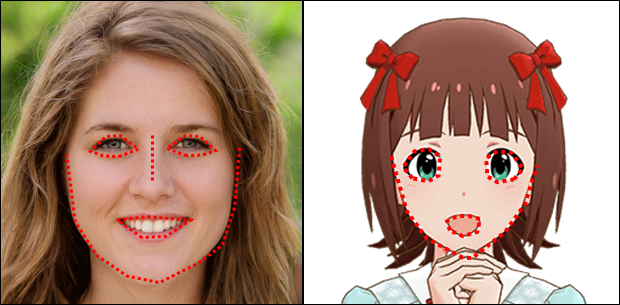
\includegraphics[width=\columnwidth]{featured_compare.png}}
\caption{Features in real-human faces and artificial human faces.}
\label{icml-historical}
\end{center}
\vskip -0.2in
\end{figure}

Most of the Japanese animations show these features. Characters in Japanese animations are often drawn without noses or lips, or even other important traits. This aspect, however, makes it an interesting target to be analyzed, as it means that machine can only be concerned with less traits than real-human faces.

In this project will step further by recognizing the emotion of anime face, using same methodology used in real-human faces.

\section{Abstract Methodology}
\subsection{Aims}
This project aims to detect faces and distinguish their expressions in Japanese-animation style, in real-time.

\subsection{Comparisons with State-of-the-Art Technology}
YOLO is a real-time object detection model based on CNN.
Based on YOLO model customization, there is a prior example of real-time Japanese animation faces and eyes detection\cite{peter2017darkflow}.

But, They lack in diversities in what to do with their model: they stayed in detecting what the faces and eyes are in the animations.
Thus, this project presents another way to use YOLO model.

\subsection{Dataset}
The dataset consists of thousands of PSD files labeled by Photoshop. PSD files include pictures of faces in japanese-animation style, layers representing the location of their eyes and facial characteristics.

\subsubsection{From Animation}
The images for dataset will be mainly collected by capturing Japanese animations.
Image will be selected by slicing animations with 15 second interval and removing redundant images that shows the same situation. It is expected to get about 4~5 images per minute.
For the sake of drawing style consistency, certain animations from the 2~3 productions will be used. The total dataset is estimated to include approximately 1500~ images, which could be added more for higher accuracy.

The listed animations will be included in the first dataset.
\begin{itemize}
\item \it{Myriad Colors Phantom World, Kyōto Animation}
\item \it{Free! Dive to the future, Kyōto Animation}
\item \it{Miss kobayasshi's Dragon Maid, Kyōto Animation}
\item \it{Tsurune: Kazemai Kōkō Kyūdō-bu, Kyōto Animation}

\item \it{Everything becomes F, A-1 Pictures}
\item \it{Magi, A-1 Pictures}
\item \it{Darling in the Franxx, A-1 Pictures}
\item \it{The Idolm@ster, A-1 Pictures}
\item \it{The Idolm@ster SIDE M, A-1 Pictures}
\item \it{The Seven Deadly Sins, A-1 Pictures}
\item \it{Working!!, A-1 Pictures}
\item \it{Sword Art Online, A-1 Pictures}
\end{itemize}

\subsubsection{From Web}
For diversities in datasets, the data will also be crawled from image databases, such as Pixiv or Danbooru.

\subsubsection{Image Selecting Rule}
Prior to model training, the data needs to be refined, since some data could lead to inhibiting training process. For this reason, data including non-human formations(ex. deformation) will be excluded. Still, images not having human formations will be used to the small extent, for they are somewhat essential for model training, but excessive amount of such data hinders training process.

\begin{figure}[ht]
\vskip 0.2in
\begin{center}
\centerline{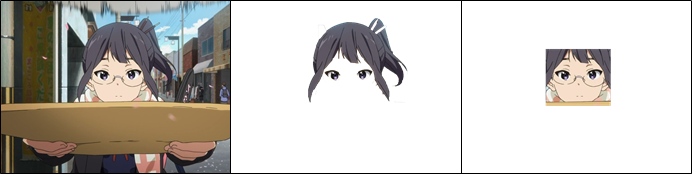
\includegraphics[width=\columnwidth]{labeling.png}}
\caption{An example of labeling pictures.}
\label{icml-historical}
\end{center}
\vskip -0.2in
\end{figure}

\subsubsection{Labeling Rule}

Additional information like facial expressions is expected to be labelled manually in the form of layers in PSD files. From this manual process of labeling, this project assumes several rules for labeling:
\begin{itemize}
\item the human should not be in deformed form.
\item Do not label accessories such as hats or glasses \newline
\end{itemize}

Following list of labels will be used:
\begin{itemize}
\item (id)\_hair
\item (id)\_eyeL
\item (id)\_eyeR
\item (id)\_emote\_(anger$|$contempt$|$disgust$|$fear\newline$|$happiness$|$neutral$|$sadness$|$suprise)
\end{itemize}

\subsection{Environment}
\subsubsection{Framework}
\begin{itemize}
\item Python 3.6.8
\item Pytorch 1.3.0a0
\item Jupyter with remote access
\end{itemize}

\subsubsection{Machine}
Machine 1 (Remote)
\begin{itemize}
\item CPU : Intel(R) Core(TM) i5-4670 CPU
\item Memory : 24GB DDR3
\item GPU : 2 x Radeon Vega Frontier Edition
\end{itemize}

Machine 2 (Local)
\begin{itemize}
\item CPU : AMD Ryzen 3600
\item Memory : 16GB DDR4
\item GPU : NVIDIA RTX 2070 Super
\end{itemize}

\section{Schedule}
\begin{itemize}
\item \emph{Oct. Week 2--Oct. Week 3} \newline Picture Crawling, Dataset Recoginition
\item \emph{Oct. Week 4--Oct. Week 5} \newline Model Design, Decision
\item \emph{Nov. Week 1--Nov. Week 3} \newline Model Training, Adjustment
\item \emph{Nov. Week 4--} \newline Result Analysis, Testing, Document Works
\end{itemize}

\section{Rule}
Kim Taehoon : Dataset Crawling \& Labeling, Model Design \newline
Ban Yonghyu: Dataset Crawling \& Labeling, Model Design \newline
Park Jinseok: Dataset Crawling \& Labeling, Result Analysis \newline
Lee Junsu : Dataset Crawling \& Labeling, Document works \newline
Yeu JaeHwang : Dataset Crawling \& Labeling, Result Analysis \newline

\bibliography{proposal.bib}
\bibliographystyle{icml2019.bst}

%\section{Reference}
%[emotion recognization]
%https://www.microsoft.com/en-us/research/wp-content/uploads/2016/02/icmi2015\_ChaZhang.pdf
%https://www.cs.ccu.edu.tw/~wtchu/papers/2017ICMR-chu2.pdf
%[yolo v1]https://pjreddie.com/media/files/papers/yolo\_1.pdf
%[yolo v2]https://pjreddie.com/media/files/papers/YOLO9000.pdf
%[yolo v3]https://pjreddie.com/media/files/papers/YOLOv3.pdf
%[yolo homepage]https://pjreddie.com/publications/


\end{document}



